\chapter{Concept And Design}\label{cap:CnptDsng}

\section{Arquitetura Geral}\label{sec:arqgrl}
\lipsum[5]
\begin{figure}[h]
	\centering
	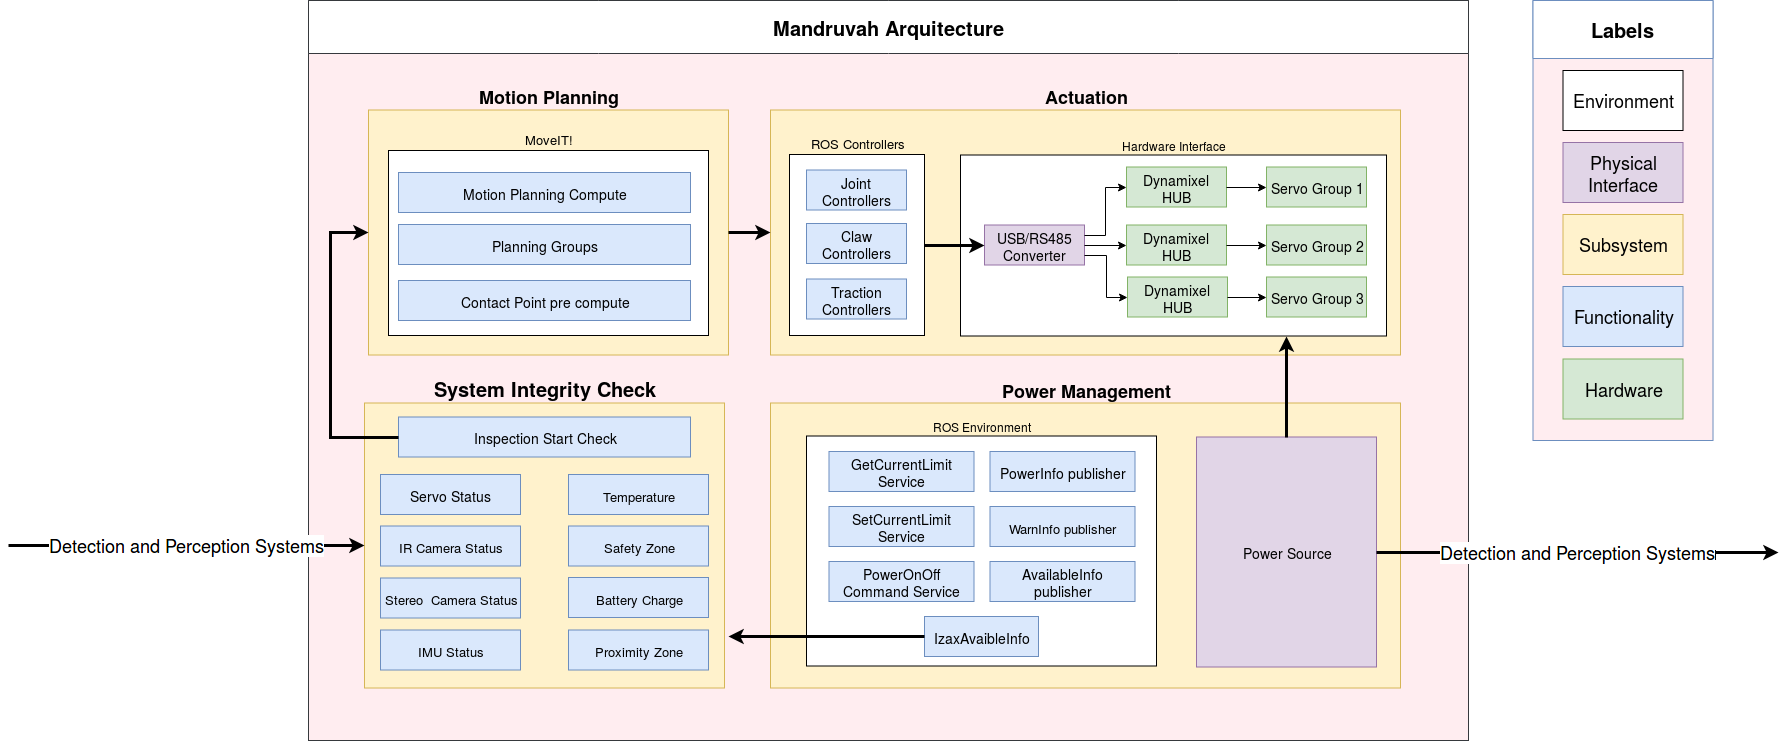
\includegraphics[width=1\textwidth]{Arquitetura.png}
	\caption{Arquitetura Geral do sistema de movimentação}
	\label{fig:arq_geral}
	\source{Própria}
\end{figure} 
\lipsum[5]


\section{Especificação Funcional}
\lipsum[3]

\subsection{Motion Planning}
\subsubsection{Definição da funcionalidade}
\lipsum[3]
\subsubsection{Dependências}
\lipsum[5]

\subsubsection{Premissas Necessárias}
\lipsum[1]
\begin{itemize}
	\item \lipsum[1]
	\item \lipsum[1]
	\item \lipsum[1]
\end{itemize}
\subsubsection{Descrição da Funcionalidade}
\lipsum[5]

\begin{figure}[h]
	\centering
	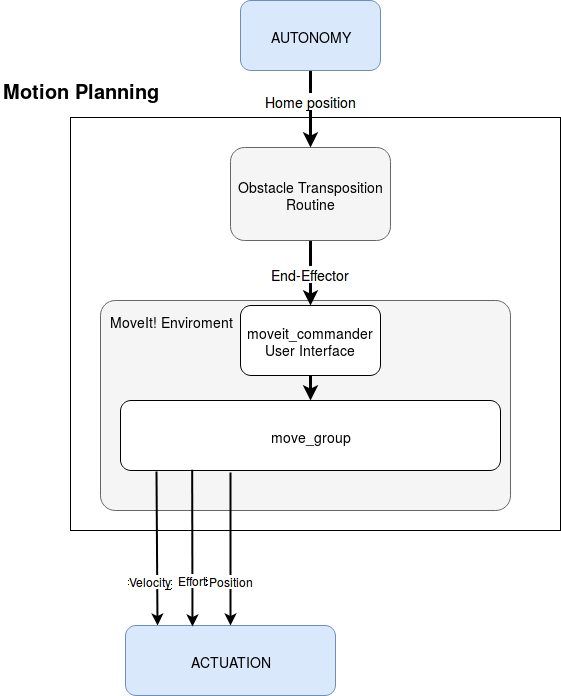
\includegraphics[width=0.6\textwidth]{motion_plan_func.png}
	\caption{Fluxograma de funcionamento da funcionalidade de Motion Planning}
	\label{fig:flux_motion}
	\source{Própria}
\end{figure}

\subsubsection{Saídas}
Por meio da compatibilização do \gls{moveit} com o \ref{itm:ros}, a saída dessa funcionalidade são os comandos de velocidade, esforço e posição para cada junta do robô.
\subsection{Actuation}
\subsubsection{Definição da funcionalidade}
\lipsum[2]
\subsubsection{Dependências}
\lipsum[5]

\subsubsection{Premissas Necessárias}
Para o correto funcionamento desse módulo, devem ser consideradas as seguintes premissas:
\begin{itemize}
	\item \lipsum[1]
	\item \lipsum[1]
	\item \lipsum[1]
\end{itemize}
\subsubsection{Descrição da Funcionalidade}
\lipsum[5]
	\begin{figure}[h]
		\centering
		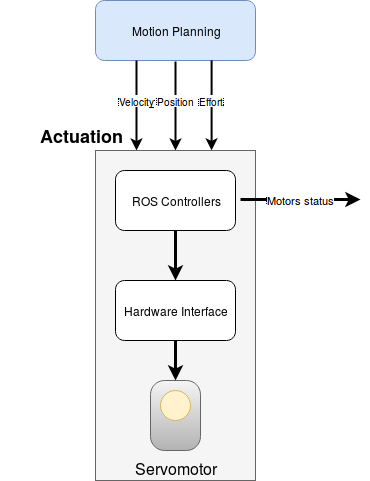
\includegraphics[width=0.6\textwidth]{actuation_depen.png}
		\caption{Fluxograma da funcionalidade Actuation}
		\label{fig:depen_actuation}
		\source{Própria}
	\end{figure}
\subsubsection{Saídas}
\lipsum[2]












